\documentclass[tikz,border=6pt]{standalone}
\usepackage{pgfplots}
\usepgfplotslibrary{groupplots}
\usetikzlibrary{calc}
\pgfplotsset{compat=1.18}
\begin{document}
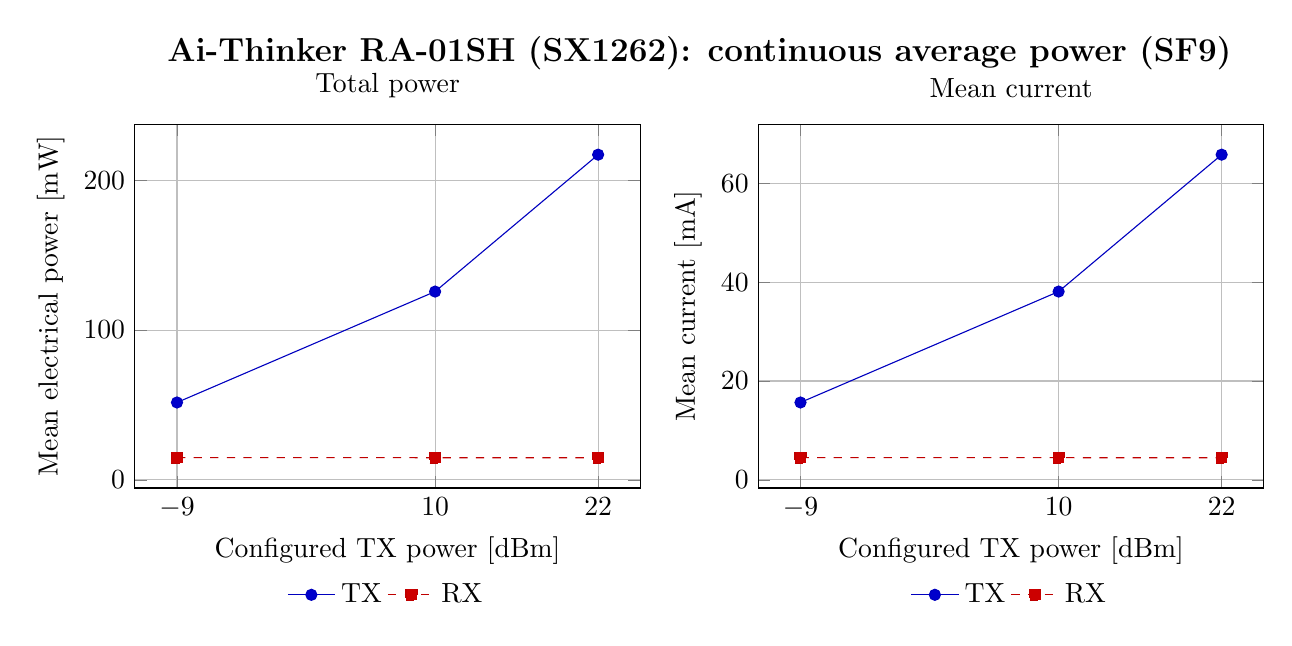
\begin{tikzpicture}
\begin{groupplot}[group style={group size=2 by 1,horizontal sep=1.5cm},width=8cm,height=6.2cm,xtick={-9,10,22},xlabel={Configured TX power [dBm]},grid=both,legend style={draw=none,at={(0.5,-0.23)},anchor=north,legend columns=2}]
\nextgroupplot[title={Total power},ylabel={Mean electrical power [mW]}]
\addplot+[blue!75!black,mark=*] coordinates {(-9,51.6376945) (10,125.698126) (22,217.114251)};\addlegendentry{TX}
\addplot+[red!75!black,dashed,mark=square*] coordinates {(-9,14.8050006) (10,14.768285) (22,14.7595442)};\addlegendentry{RX}
\nextgroupplot[title={Mean current},ylabel={Mean current [mA]}]
\addplot+[blue!75!black,mark=*] coordinates {(-9,15.6477862) (10,38.0903411) (22,65.7921974)};\addlegendentry{TX}
\addplot+[red!75!black,dashed,mark=square*] coordinates {(-9,4.48636382) (10,4.47523789) (22,4.47258914)};\addlegendentry{RX}
\end{groupplot}
\node[font=\bfseries\large] at ($(group c1r1.north)!0.5!(group c2r1.north)+(0,0.9cm)$) {Ai-Thinker RA-01SH (SX1262): continuous average power (SF9)};
\end{tikzpicture}
\end{document}
